\subsection{Photolithography}
\label{sec:lithography}

%\begin{figure}[h]
%    \centering
%    \includegraphics[width = 0.8\textwidth]{figures/chapter2/litho/Fig8_litho.pdf}
%    \caption{}
%    \label{fig:litho}
%\end{figure}

Photolithography is an ancient technique that uses light (usually ultraviolet) to very precisely transfer a pattern onto a substrate, and is often used to create the very small structures typical of electronics. The EG-FET fabricated in this project is no exception.

The photolithography process began by thoroughly cleaning the polyimide (PI) substrate by leaving it for \SI{5}{\min} in an ultrasound bath in acetone, followed by an ultrasound bath in isopropyl alcohol for additional \SI{5}{\min}.
Then, the substrate was dried in an oven for \SI{24}{\hour} at \SI{200}{\celsius}, with the aim of removing any residual moisture and solvents. This procedure ensured that the surface was uncontaminated and ready for the following steps.

After cleaning, the substrate underwent a pre-baking step on a hotplate at \SI{115}{\celsius} for \SI{5}{\minute}, followed by \SI{5}{\minute} in a 
To further prepare the substrate, it was exposed \SI{5}{\minute} to hexamethyldisilazane (HMDS) environment, where the resulting vapour reacts with the surface, forming a hydrophobic layer and preventing moisture formation, which could interfere in the subsequent adhesion between the substrate and the photoresist \citep{pollentierBake2022}.

Photoresist was then deposited using a spin coater; the thickness and uniformity was controlled by appropriately adjusting the speed and time of rotation.
It is now important to note that photoresists are categorized as positive and negative, depending on how the solubility changes upon light exposure. Indeed, in positive photoresists, like AZ 1518, light exposure causes polymer chains to break down, making the exposed areas more soluble in the developer. When he exposed regions are removed, they leave a pattern corresponding to the mask. For negative photoresists, like ma-N 1420, the one used in this project, UV exposure cross-links polymer chains, making the exposed areas less soluble in the developer. The unexposed regions are subsequently removed, leaving the inverse pattern of the mask.

After photoresist deposition, the substrate underwent post-baking on a hotplate at \SI{100}{\celsius}; this step was needed to stabilize the photoresist layer and to improve its chemical resistance for later steps, ultimately ensuring high resolution patterning during UV exposure and development \citep{miyajimaHighaspectratio1995}.

The substrate with the photoresist was then aligned with a photomask containing the desired pattern. UV light was used to expose the photoresist through the mask, transferring the pattern onto it. The exposure dose was set to \SI{279.48}{\mJ/\cm\squared} to ensure proper resolution and pattern fidelity.

After exposure, the substrate underwent development to remove the unexposed areas of the photoresist. MA-D533/S developer, an aqueous-alkaline surfactant containing tetramethylammonium hydroxide (TMAH), was chosen for its compatibility with the ma-N 1420 photoresist. The PI substrate was left in the developer bath for \SI{2.5}{\minute}, then thoroughly rinsed with abundant \ce{diH2O}, ensuring optimal resolution and edge definition of the developed pattern.

\subsection{Electrode deposition}
\label{sec:eavporation}

After photolithography, multiple techniques can be used to deposit the electrodes, including physical vapour deposition (PVD) techniques. This term refers to those methods where the target material (\eg{} a metal) is processed in such a way that it changes phase, namely from solid to vapour, and then to solid again (no reactions occur during the phase changes). Two common PVD techniques are sputtering, where high-energy ions bombard the target causing the atoms to detach, evaporate and reattach on the substrate, and evaporation, where the target is heated enough to have the metal evaporate, deposit on the substrate and solidify again, mostly in the form of thin film. In the case of this project, the choice fell on evaporation for practical reasons: the evaporator was simply already setup for the process, offering the possibility to evaporate both the titanium adhesion layer and the actual gold electrode. This process also allowed to tightly control the thickness of the electrodes and produced very uniform metal surfaces. As a PVD technique, it is important to notice that evaporation occurs in vacuum conditions (\SI{<2e-6}{\mbar}): this helps in removing vapours other than the metal and prevents impurities from contaminating the surface. First, an adhesion layer of \SI{10}{\nm} of titanium was deposited. Since titanium has a high-melting point (\SI{1668}{\celsius}), an electron beam (e-beam) was necessary to sufficiently heat up the metal: in this process, a metal filament is electrically charged (a current of approximately \SI{100}{\mA} was applied) to the point where it releases electrons; these same electrons are emitted with very high energy and on a very focused spot that gets heated up until it starts to evaporate. These vaporized atoms then land on a cold surface, \ie{} the substrate, where they condense again, forming the thin layer needed for gold to adhere to the substrate. Indeed, without this, gold would be more prone to delamination or chipping, at the risk of making our efforts invain. Next, a \SI{50}{\nm} gold layer was deposited using thermal evaporation. This method relies on resistive heating to reach the melting point of a gold pellet (\SI{1064.18}{\celsius}), which then evaporates and travels in the chamber until it condenses on the PI surface, which is now covered in titanium. For both processes, it was imperative to maintain the evaporation rate as stable as possible, in order to deposit a uniform layer with minimal defects. This would then favour stability in the fabricated devices; the best results were obtained when evaporating at a rate between \SIrange{0.2}{0.5}{\angstrom\per\second}. To also contribute to the uniformity of the deposited layers, the substrate was placed on a rotating support, which promoted an even distribution of the evaporated material. After metal deposition, the lift off process took place by immersing the substrate (now fully covered in metals, without any pattern visible) in acetone for \SI{60}{\min}; indeed, ma-N 1420 is sensitive to acetone, which can be used to remove the excess. After the acetone bath, the substrates were placed in an ultrasound sonicator for few seconds, then rinsed with a bottle. This process was repeated 3 times with acetone and once with IPA to ensure that all remaining photoresist was removed, and the overlaying metals with it. The devices were then dried with an air gun and checked for any fabrication defects, \eg{} gold speckles in the channel that could later cause short circuits.

%\begin{figure}[h]
%    \centering
%    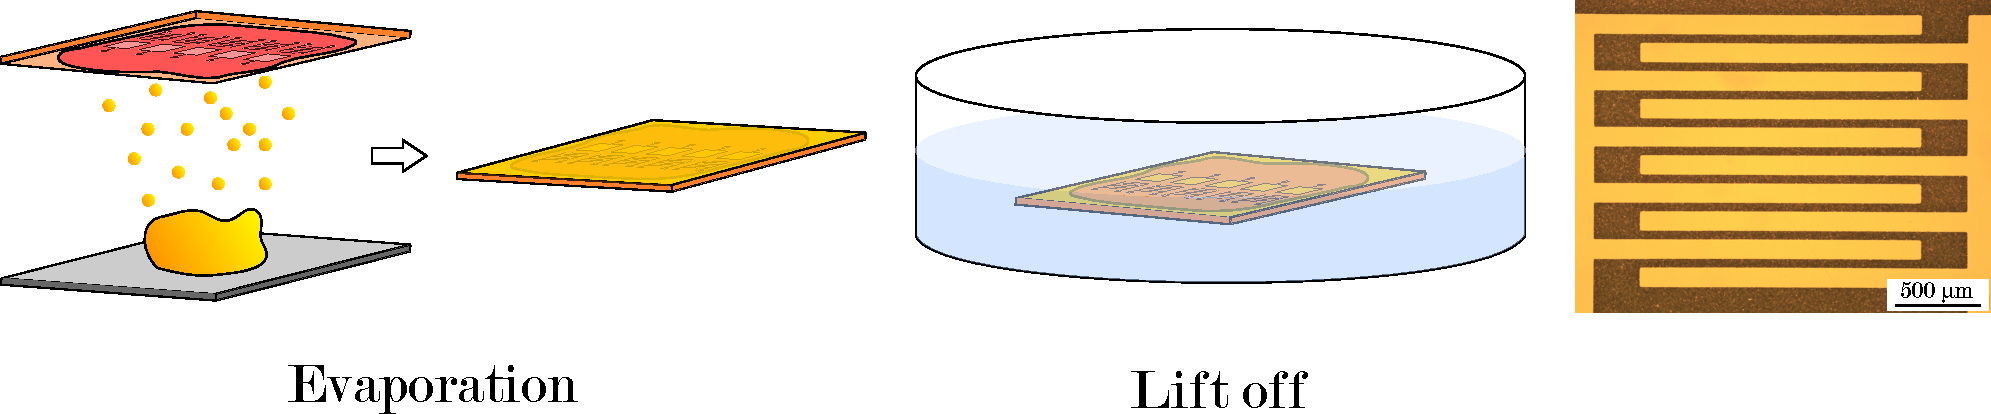
\includegraphics[width=0.8\textwidth]{figures/chapter2/litho/Fig9_evap.pdf}
%    \caption{}
%    \label{fig:evap}
%\end{figure}
